% !TEX root = ferguson-dissertation.tex

\chapter{Interacting with \sys}
\label{sec:messages}

We now expand upon the three message types introduced
in the overview: requests, queries, and hints. Table~\ref{tab:concepts}
has a concise specification of these messages, and their
relation to other key concepts in \sys.

%Shares and the share tree do not affect the network
%themselves. Instead, \sys maintains a second data-structure, the
%\emph{policy tree}, which determines network-wide policy.  \sys
%ensures two key invariants. First, it ensures that the policy tree
%always has the same tree-structure as the share tree. Second, it
%ensures that all \emph{policy atoms} in a policy tree node are authorized by
%the corresponding share.
%
%Each node in the policy tree holds a set of policy atoms, which we write
%as follows:
%\[
%  \paneprin{user}{host}{app}:\{F\}\rightarrow\panemsg
%\]
%A policy atom indicates that a principal affects a flowgroup in the
%manner determined by \panemsg, which we describe below.

\section{Requests}
\label{sec:Requests}

A \emph{request} affects the state of the network for some interval of time. 
%{\color{red} When \sys receives a request, it first checks that the principal
%has the necessary privileges in the share tree. Second, it checks if
%the request can co-exist with previously accepted requests by checking
%the policy tree for the start and end times, as we will describe in
%\Cref{sec:PolicyTrees}. }
%
By default, requests take effect immediately and do not expire;
specific start and end times may optionally be provided.  Verifying if
a request can be granted may require walking the tree's hierarchy,
depending on the type of request.  This design allows resources to be
oversubscribed; overallocation is prevented when requests are granted,
and not when shares are created.

Participatory networks may support requests for a variety of network
resources and services, which we detail next.

\tightparagraph{Access Control}
The simplest type of network service exposed by \sys is access control
-- the ability to allow and deny traffic, using the \textbf{Allow} and
\textbf{Deny} requests.  Like all requests, they specify a flowgroup
describing the affected traffic, and the share which the principal is
using to invoke the privilege.
Each access control privilege is optionally constrained by a specified
number of seconds, $n$.
To exceed this limit, principals must periodically renew requests.
Shares lacking the ability to allow or deny traffic have $n = 0$.
When creating a sub-share, a principal cannot exceed these constraints. For example,
if a share carries the privilege to \priv{Deny} traffic for up to
300 seconds, a sub-share cannot be created with the privilege to \priv{Deny}
traffic for up to 301 seconds; similarly, a sub-share could not be created
with the privilege to \priv{Allow} traffic.

The handling of a given packet is ultimately decided by the
composition of every matching access control request. This composition
makes use of the share tree's hierarchy to resolve conflicts -- for
example, an access control request made on a child share overrides
those in parent shares.  We defer further discussion of \sys's general
approach to conflict resolution until
\Cref{sec:conflicts}.

With each request, the principal can specify a fulfillment mode, either
\emph{strict} or \emph{partial}. These are provided for atomicity and
convenience. In strict mode, \sys rejects a request if it would be
(partially) overridden by any previous request.
%optional example
For example, if a user wants to allow connections to TCP ports
1000-2000, but there exists a request in a sub-share that denies port
1024, \sys rejects the request, explaining why.  In partial mode, \sys
implements the request, and informs the user that it was only
partially satisfied;
%optional example
in the same example, \sys would inform the user that it has allowed
ports 1000-1023, and 1025-2000.

These modes exist for two reasons: first, to avoid race conditions in
request allocations, and second, to avoid complicated, fine-grained
specifications that depend on \sys's current state. We defer a more
complete discussion of the strict and partial fulfillment modes until
\Cref{sec:strict-partial}.

\begin{figure}[t]
\centering
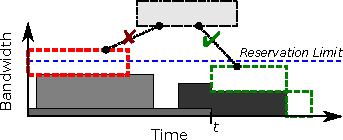
\includegraphics[width=0.6\textwidth]{figs/sched}
\caption{Example user request for reserved bandwidth;
\sys determines that it cannot be fulfilled until time $t$.}
\label{fig:sched}
\end{figure}


\tightparagraph{Guaranteed Minimum Bandwidth}
\sys also provides a \priv{Reserve} privilege which provides
guaranteed minimum bandwidth (GMB) between two hosts.
Shares which contain the privilege to reserve bandwidth are limited
by a modified token bucket:
it has the usual attributes of fill rate $F$, capacity $C$, and maximum
drain rate $M$, and an additional minimum drain rate $m$. This lower
bound prevents reservations with very low drain rates that could
last indefinitely. A simple reservation with maximum
bandwidth $B$ is a special case with $F = M = B; C = m = 0$. GMB
reservations are ultimately implemented by \sys's runtime as a
sequence of forwarding actions and switch queues, as we describe in
\Cref{sec:FullSystem}. Requests which cannot be implemented are
rejected.

Figure~\ref{fig:sched} shows a simple example in which a principal
has requested an immediate bandwidth reservation. \sys determines
that granting the request will exceed the share's available bandwidth.
The principal then examines the share's schedule of available bandwidth
and sends a new request for a reservation
to start at $t$; \sys accepts the request and later implements it.

When creating sub-shares of shares with GMB privileges, the sub-share's
token bucket must ``fit inside'' the parent's token bucket; parents cannot
provide more tokens to their children than they receive. However, a share's
tokens can be over-subscribed by its sub-shares. When a request is granted,
it draws tokens from all of its parent shares, up to the root of the tree, thus
preventing over-allocation.

\tightparagraph{Path Control}
A third request type directs flows through or around middleboxes using
\priv{Waypoint} and \priv{Avoid}.
For example, a university's network administrators can
route students' traffic through a packet shaper during business hours,
and security researchers can avoid intrusion detection systems for traffic to be collected by honeypots.
Shares contain sets of IP addresses listing the middleboxes which
they can route through or avoid, and, as with flowgroups, sub-shares may
only contain subsets of their parents' sets.
\sys implements \priv{Waypoint} and \priv{Avoid} by installing flow-specific
forwarding rules along a path determined by
fixing or deleting nodes as appropriate when routing over the network graph
(\Cref{sec:NIB}). Requests to create unrealizable paths are rejected.

\tightparagraph{Rate-limits}
\sys supports rate-limit requests which result in matching traffic 
being routed through
ports with established rate-limiters, as available in current switches.
While basic, such requests can be used to mitigate DOS attacks or
enforce traffic contracts between tenants in a shared datacenter.
\sys's global view of the network enables it to make best use of the switches'
features and place rate-limiters close to the traffic's source, as we describe in \Cref{sec:NIB}.
Like \sys's bandwidth reservations, rate-limits are currently restricted to circuits;
a network with distributed rate-limiters, such as those proposed
by Raghavan, \etal~\cite{Raghavan:2007}, could support more general limits.
Their integration is left as future work.

\section{Queries}
\label{sec:Queries}

\sys also supports messages to query the state of the network.
These queries may be for general information about the network,
such as the type of a link (\eg, copper or optical), the set of hosts
located downstream of a particular port, or other properties.
Each share may contain a list of properties which it is privileged
to read. This list is similar to a ``view'' on a database; when sub-shares
are created, this view may be further occluded. While these restrictions
provide basic privacy protection when exposing the network's state,
they are not complete. For example, if a switch has three links, and
a principal has the privilege to read the sending and receiving rates
on two of the links, but not the third, it can infer the rate on the third link.
We leave a more complete development of privacy protections as
future work.

The current OpenFlow specifications and design make a number of
properties available which principals in \sys may query including:
 the number (or list) of hosts behind a particular
port, port-specific diagnostic data such as the number of packets
dropped, the number of CRC errors, etc., the physical and topological
location of switches, and the access medium of links. In the future,
we would like to support additional details we believe would
benefit applications such as the current signal-to-noise ratio or
broadcasting power of wireless access points.

\sys also supports a ``network weather service'' which provides coarse
information about current traffic conditions. For example, statistics
about the total amount of traffic over a core link are available, but
not statistics about individual flows. By integrating \sys with a
project like Frenetic~\cite{Foster:2010}, we expect it could support
the ability to query the traffic statistics of individual flows, as
such queries require a more robust OpenFlow runtime than our current
implementation.

Applications can issue queries to the \sys controller to improve the
user experience. For example, Hadoop could use the weather service to
place reducers away from currently-congested parts of the network, and
streaming video players can determine that a wireless access point is
attached to a cellular modem or similarly constrained backhaul as
Shieh, \etal proposed~\cite{Shieh11netquery}.

\section{Hints}
\label{sec:Hints}

The final type of message in \sys is a hint. Hints are used to provide
the network with information which may improve the application's or
network's performance, without creating an additional
requirement. Providing hints across abstraction boundaries is a
natural feature in other systems.
For example, if a three-tier web application makes
a request to the database layer, and hints to the caching layer that it
won't make the same request again in the near future, the cache may
choose to skip storing the result.

Three hints which are useful for networked applications include: the
size (in bytes) of a flow, a desired flow-completion deadline, and the
predictability of future traffic. \sys can use flow size information
to spread large flows across multiple paths of equal-cost, as in Mahout~\cite{curtis11mahout} or
Hedera~\cite{alfares10hedera}.  Deadlines
can be communicated to supporting routers such as those proposed in
D3~\cite{wilson11d3}. And hints about traffic predictability can be
used by traffic optimizers such MicroTE~\cite{Benson2011microte}.

\sys \emph{may} use hints to derive and install policy atoms which affect
related traffic, although it gives no guarantee or notification to the user. 
For example, a hint that a flow is short may generate
a policy atom to increase that flow's priority. We call such hints
\emph{realized}, and their corresponding policy atoms are tagged as
merely hints (\cf Table~\ref{tab:concepts}).

The integration of hints, which can benefit non-\sys systems, as in
the examples above, is deliberate. \sys provides a network
administrator with the framework to delegate privileges, divide
resources, and account for their usage; the ability to issue hints is
a privilege, particularly those which affect limited resources.  The
framework provided by \sys makes it more feasible to implement hints
in an untrusted environment, where malicious principals may issue
false or excessive hints in an attempt to gain an advantage.

Finally, in the absence of transactional-style requests (\eg, a
request for ``resource A \emph{or} resource B''), \sys's hints are a
more flexible way to provide information to the network than via
requests. In this use, hints share a similar role to \sys's partial
fulfillment mode for requests (\Cref{sec:strict-partial}).

\begin{comment}
Hints are not promises, and can always be ignored by the \sys controller. The 
two best examples we have so far are:
\begin{enumerate}
\item ``This is an RPC'' -- it will be short and should have low-latency.
\item ``Size of flow'' hint -- this came up in our discussion with Scott Shenker,
where it would be useful for queues in a switch or spreading elephants across
multiple links.
\item ``Predictable traffic'' hint -- useful for something like Theo's MicroTE~\cite{Benson2011microte}
\end{enumerate}
\end{comment}

\begin{landscape}
\begin{table*}
\centering 
\begin{small}
\[
\begin{array}{ll@{\,}c@{\,}ll}
\hline
\textrm{Share} & S & \in & 
%
\{P\} \times \{F\} \times \{ \panepriv \} & 
%
  \textrm{A share gives principals some privileges to
    affect a set of flows.} \\
%
\textrm{Principal} & P & \mathord{::=} &
%
\paneprin{\textrm{user}}{\textrm{host}}{\textrm{app}} &
% 
  \textrm{A triple consisting of an \emph{application}, running on a
    \emph{host} by a \emph{user}.} \\
%
\textrm{Flow} & F & \mathord{::=} & \langle\textbf{srcIP}\mathord{=}n_1,\textbf{dstIP}\mathord{=}n_2, &
%
  \textrm{A set of packets with shared properties: source and destination IP address,} \\
%
& & & \quad\textbf{proto}\mathord{=}n_3,\textbf{srcPort}\mathord{=}n_4,\textbf{dstPort}\mathord{=}n_5\rangle &
%
  \qquad\textrm{transport protocol, and source and destination transport ports.}\\
%
\textrm{Privilege} & \panepriv & ::= &
%
\textbf{CanDeny}~n \mid \textbf{CanAllow}~n &
%
\textrm{The privileges to allow or deny traffic for up to $n$ seconds (optional).} \\
%
& & & \mid \textbf{CanReserve}~n \mid \textbf{CanRateLimit}~n & 
%
  \textrm{The privileges to reserve bandwidth or set rate-limits, up to
    $n$ MB.} \\
 %
& & & \mid \textbf{CanWaypoint}~\{\textit{IP}\}\mid \textbf{CanAvoid}~\{\textit{IP}\} & 
%
  \textrm{The privileges to direct traffic through or around particular IP addresses.} \\
\hline
%
\textrm{Message} & \textit{Msg} & \mathord{::=} &
%
P:\{F\} : S \rightarrow ( \panereq~\panetspec \mid \panehint~\panetspec \mid \panequery) &
%
\textrm{A message from a principal with a request, hint, or query using a share.} \\
%
\textrm{Time Spec} & \panetspec & ::= & \textbf{from}~t_1~\textbf{until}~t_2 &
%
\textrm{An optional specification from time $t_1$ until $t_2$.} \\
%
\textrm{Request} & \panereq & \mathord{::=} & 
%
\textbf{Allow} \mid \textbf{Deny} &
%
\textrm{Request to allow/deny traffic.}
\\
%
& & &  \mid \textbf{Reserve}~n \mid \textbf{RateLimit}~n~ &
%
  \textrm{Request to reserve $n$ MB or rate-limit to $n$ MB.} \\
%
& & & \mid \textbf{Waypoint}~\textit{IP} \mid \textbf{Avoid}~\textit{IP} &
%
\textrm{Waypoint/avoid traffic through a middlebox with the given IP address.} \\
%
\textrm{Query} & \panequery & \mathord{::=} &
%
\textbf{TrafficBetween}~\textit{srcIP}~\textit{dstIP} \mid ... &
%
\textrm{Query the total traffic between two hosts.} \\
%
\textrm{Hint} & \panehint & \mathord{::=} &
%
\textbf{Duration}~t \mid ... & \textrm{Hint that the flow's duration is $t$.} \\
%
\textrm{Policy Atom} & \panepolatom & \mathord{::=} & 
%
P:\{F\} \rightarrow \panereq~\panetspec &
%
\textrm{A requested modification of network state.} \\
%
& & \mid & \textbf{Hint}~P:\{F\} \rightarrow
\panereq~\panetspec &
%
\textrm{A realized hint; it may be removed if it conflicts with a future request.} \\
\hline
\end{array}
\]
\end{small}
\caption{Main concepts in \sys}  \vspace{-1em}
\label{tab:concepts}
\end{table*}

\end{landscape}

\chapter{Privilege Delegation in \sys}
\label{sec:delegation}

\begin{figure}[t]
\centering
\subfigure[]{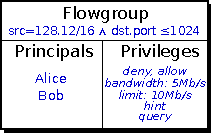
\includegraphics[width=0.35\textwidth]{figs/share}}\hfill
\subfigure[]{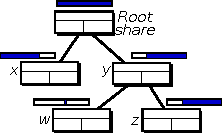
\includegraphics[width=0.35\textwidth]{figs/sharehierarchy}}
\caption{(a) A \sys share. (b) A share
hierarchy. The rectangle above each share represents a flowgroup
according to one dimension (\eg, source IP). Sub-shares are defined
on a subset of their parent's flowgroup, and may not have more permissive
privileges than their parent.}
\label{fig:shares}
\end{figure}

%\vskip 1em

This chapter presents the semantics of shares and how principals'
messages are authorized in more detail. The \sys
controller maintains two key data structures. First, the \emph{share
  tree} determines the privileges that principals have to read or write
  network state. The tree-structure allows principals to create new shares and
delegate authority to each other. The share tree itself does not
affect the state of the network. Instead, the second key
data-structure, the \emph{policy tree}, holds \emph{policy atoms} that
can affect the network. \sys maintains the invariant that all policy
atoms in the policy tree are properly authorized by the share tree at
all times.

%\section{Share Tree\label{sec:sharetree}}
\vskip 1em

A share-tree is an $n$-ary tree of \emph{shares}, where a share gives
a set of \emph{principals} some \emph{privileges} to affect a set
of \emph{flows} in the network. We elaborate on these terms below.

\tightparagraph{Principals}
A \sys principal is a triple consisting of an application running on a
host by a user. A principal may be
\paneprin{Skype}{192.168.1.7}{Alice} or
\paneprin{Hadoop}{10.20.20.20}{Bob} for example. Shares in \sys are held by
principal-sets.  We abbreviate singleton sets to their principal. We
also use wildcards to denote large sets. \eg, \paneprinuser{Alice} is
the set of all principals with Alice as the user, and
\paneprinapp{Hadoop} is the set of all principals with Hadoop as the
application. We write \paneprinall \ to denote the set of all
principals.

Principals send messages to the \sys controller to request resources
and query the state of the network. For example, the principal
\paneprin{Skype}{192.168.1.7}{Alice} may request low-latency service
between the Skype call's source and destination, and the principal
\paneprin{Hadoop}{10.20.20.20}{Bob} may request guaranteed bandwidth
between the three machines in an HDFS write pipeline, as we implement
in \Cref{sec:ApplicationUsage}.

In a deployed system, \sys could use 802.1x to authenticate the user
portion of a principal against an existing user database such as
Active Directory or LDAP. In an ideal environment, the application and
host portions could be attested to by a TPM module and application
signatures on the end host~\cite{Nexus}.  For now, our prototype only
considers the user portion of a principal.

The three-part principal design allows users and network
administrators to fully understand the provenance of each request. For
example, in a cluster of Hadoop machines, requests by different
Application Masters are identifiable back to the specific machine they
were made from. Similarly, users can differentiate between requests from
distinct applications on the same machine.

\tightparagraph{Flows}
\label{sec:Flowgroups}
A flow is a set of related packets on which requests are
made. For example,
\[
\paneshare{w}{x}{\textit{TCP}}{y}{z}
\]
is a flowgroup that denotes a TCP connection from $w:y$ to $x:z$. A
\sys share allows principals to affect a set of flows, which we denote
with wildcards when possible. For example, the following flowgroup
denotes all HTTP requests:
\[ 
  \paneshare{\star}{\star}{\textit{TCP}}{\star}{80} 
\]
whereas the following denotes HTTP requests and responses:
\[
  \begin{array}{l@{}l}
  \paneshare{\star}{\star}{\textit{TCP}}{\star}{80} & \cup \\
  \paneshare{\star}{\star}{\textit{TCP}}{80}{\star}
  \end{array}
\]
A key invariant of the share tree is that if share $S_1$ is a
sub-share of share $S_2$, then $S_1$'s flowgroup is a subset of $S_2$'s
flowgroup. Therefore, sub-shares allow principals to implement
fine-grained delegation of control.

\tightparagraph{Privileges}
%
Privileges in \sys define the messages principals may send using the share.
Each message type, as described in the previous chapter, has a corresponding
privilege. For example,
\textbf{CanAllow}~$n$ and \textbf{CanDeny}~$n$ permit
admission-control policies to be requested for $n$ seconds, and $\textbf{CanWaypoint}~\{\textit{IP}\}$
indicates that principals can route traffic through an IP address in the given set.
